\section{Benchmark Construction and Statistics} \label{appendix:construction}
In this section, we provide more details about the process of constructing our benchmark. A sample prompt for generating functions and test cases is shown in Listing \ref{lst:benchmark-generation-prompt}. The prompt is constructed by including two few-shot examples, one containing a specified \texttt{str} function and one containing a specified \texttt{list} function. The full list of specified functions is given in \ref{appendix:benchmark-generation-functions}, and the full list of few-shot examples chosen from is given in \ref{appendix:benchmark-generation-fewshot}. We learned that having random-looking inputs instead of common words and phrases in the few-shot prompts significantly increased the difficulty of the benchmark.

\begin{lstlisting}[caption={Sample prompt for generating functions and test cases},label={lst:benchmark-generation-prompt}, captionpos=t, breaklines=true]
You will be given a function name between [TASK] and [/TASK] tags. Following the examples given, write a Python function that makes use of the given function and 5 test inputs for that function.

[TASK]
str.center
[/TASK]
[PYTHON]
def f(text):
    ls = list(text)
    for i in range(1, len(ls) - 1):
        ls.insert(i, '+')
    return ''.join(ls).center((len(ls) - 1) * 2)
[/PYTHON]
[TEST]
assert f('lynel') == ??
assert f('nzoh') == ??
assert f('u') == ??
assert f('anfsoixz') == ??
assert f('xzd') == ??
[/TEST]

[TASK]
list.append
[/TASK]
[PYTHON]
def f(nums):
    count = len(nums)
    for i in range(-count+1, 0):
        nums.append(nums[i])
    return nums
[/PYTHON]
[TEST]
assert f([2, 6, 1, 3, 1]) == ??
assert f([7, 1, 2, 6, 0, 2]) == ??
assert f([4, 3, 2, 1, 2, -1, 4, 2]) == ??
assert f([0, 6, 2, -1, -2]) == ??
assert f([-6, -2, 1, -3, 0, 1]) == ??
[/TEST]

[TASK]
str.zfill
[/TASK]
[PYTHON]
\end{lstlisting}

\subsection{Functions used in prompt} \label{appendix:benchmark-generation-functions}
For each of \texttt{str}, \texttt{list}, and \texttt{dict}, we use all the non-dunder methods under that class. The resulting list of methods is as follows:
\begin{itemize}
    \item \texttt{str}: capitalize, casefold, center, count, encode, endswith, expandtabs, find, format, format\_map, index, isalnum, isalpha, isascii, isdecimal, isdigit, isidentifier, islower, isnumeric, isprintable, isspace, istitle, isupper, join, ljust, lower, lstrip, maketrans, partition, removeprefix, removesuffix, replace, rfind, rindex, rjust, rpartition, rsplit, rstrip, split, splitlines, startswith, strip, swapcase, title, translate, upper, zfill
    \item \texttt{list}: append, clear, copy, count, extend, index, insert, pop, remove, reverse, sort
    \item \texttt{dict}: clear, copy, fromkeys, get, items, keys, pop, popitem, setdefault, update, values
\end{itemize}

Motivated by seeing a GPT-4 failure of treating the \texttt{\^} symbol as an exponential rather than an xor, we also attempted using all the non-dunder methods from \texttt{operator}. However, we found that the majority of the functions obtained were either too simple and uninteresting, or too computational, since many of the methods under \texttt{operator} are bit-manipulation or calculational operations. Therefore, we excluded it from our final benchmark.

\subsection{Few-shot Examples} \label{appendix:benchmark-generation-fewshot}
We use 10 handwritten few-shot examples, 5 using \texttt{str} functions and 5 using \texttt{list} functions. For each prompt, we include two few-shot examples, one string few-shot example and one list few-shot example, for a total of 25 different combinations of few-shot prompts. We generate programs and inputs using \codellamalarge with temperature $T=1$. 

One interesting observation is that for a fixed pair of few-shot examples, there seems to be a limit to the number of diverse functions that can be generated: after about $60000$ generations, only about $5000$ of them were unique. Using all 25 combinations of few-shot prompts helps to overcome this duplication bottleneck.

The full set of few-shot examples can be found in Listing \ref{lst:benchmark-generation-fewshot}.

\subsection{Dataset Statistics} \label{appendix:benchmark-dataset-statistics}

\label{appendix:benchmark-statistics}
In Fig. \ref{fig:dataset-distributions}, we show the distribution of character count and line count of the 800 samples in our benchmark.

\begin{figure}[H]
    \centering
    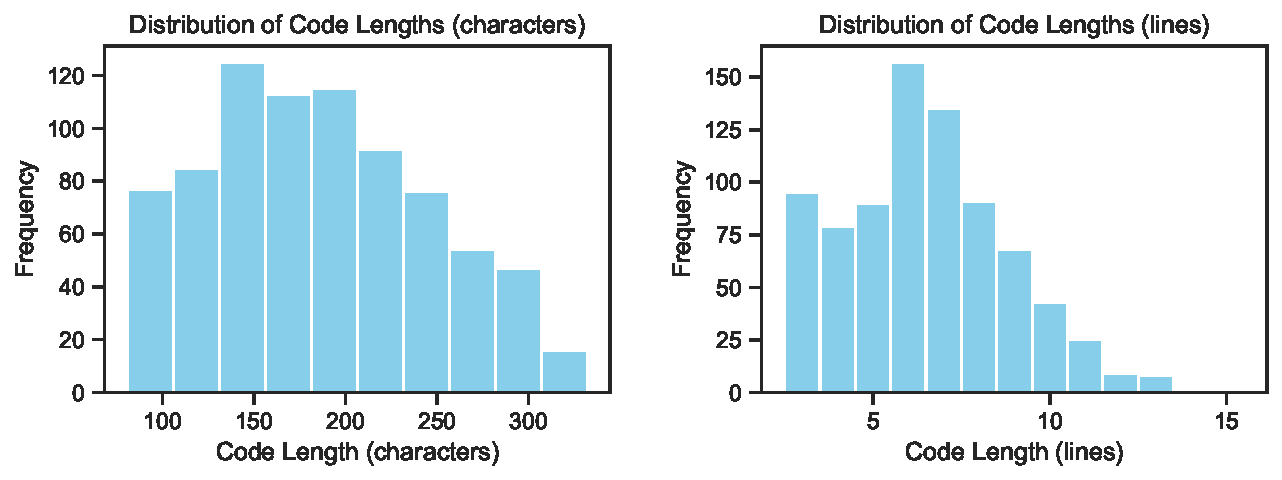
\includegraphics[width=0.9\textwidth]{figs/benchmark/dataset_distributions.pdf}
    \caption{Dataset Distributions}
    \label{fig:dataset-distributions}
\end{figure}

In Fig. \ref{fig:num-steps}, we show the distribution of the ``step count'' of programs (with one outlier of 3175 steps excluded). Here, steps roughly correspond to Python bytecode operations during execution. The precise definition can be understood by checking the ``numsteps'' variable in our code \href{https://github.com/minimario/cruxeval/blob/main/data/filter/analyze_ops.py}{here}.

\begin{figure}[H]
    \centering
    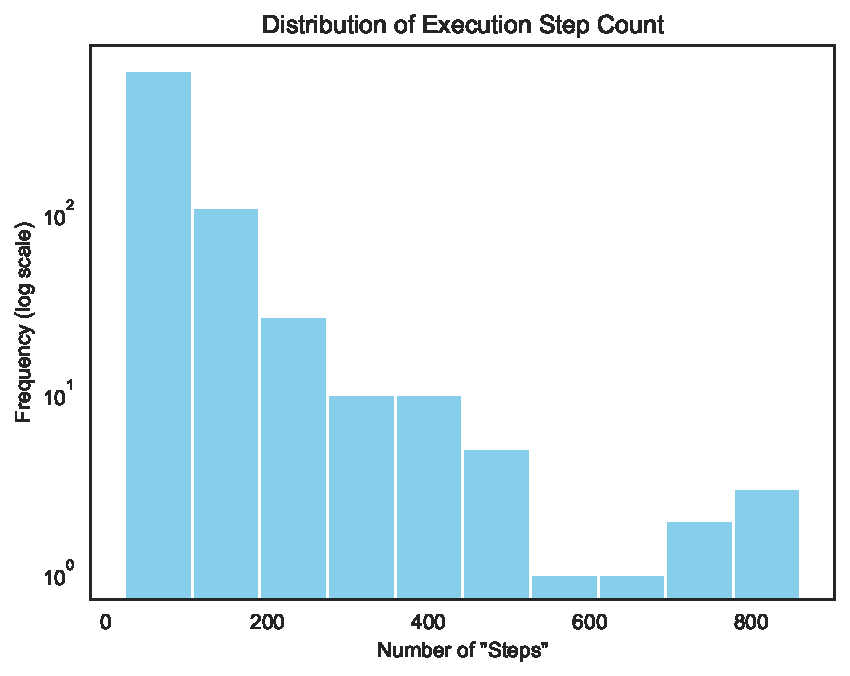
\includegraphics[width=0.5\textwidth]{figs/benchmark/num_steps.pdf}
    \caption{Number of steps}
    \label{fig:num-steps}
\end{figure}

In Fig. \ref{fig:benchmark-sample-io-correlation}, we plot the output prediction pass@1 scores against the input prediction pass@1 scores for each sample, observing little to no correlation between the difficulty of the two.

\begin{figure}[H]
    \centering
    \begin{subfigure}[b]{0.49\textwidth}
        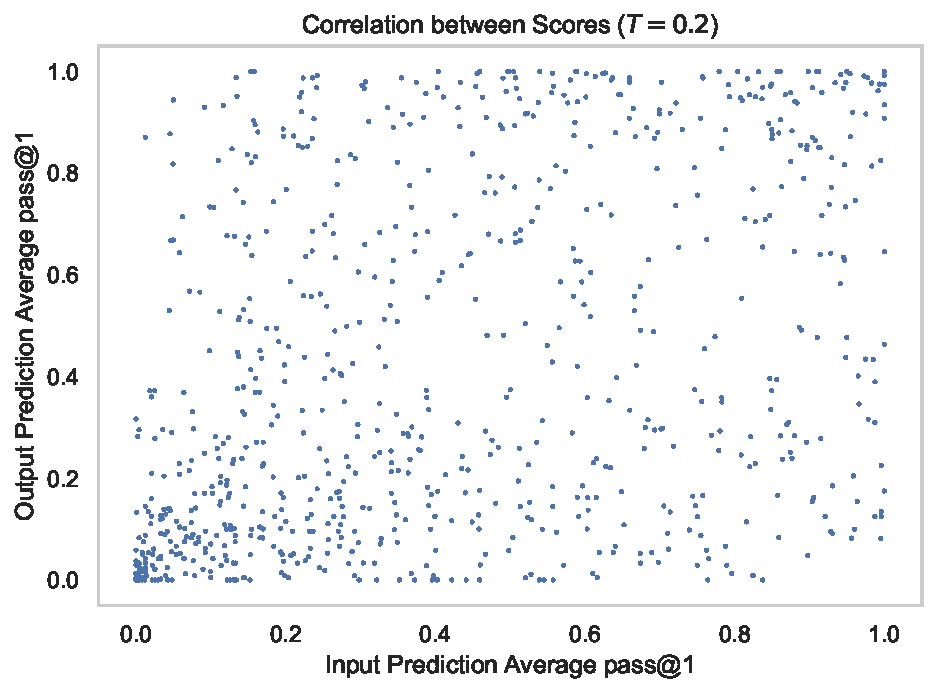
\includegraphics[width=\textwidth]{figs/benchmark/io_sample_correlation_0.2.pdf}
        \caption{$T=0.2$}
    \end{subfigure}
    \begin{subfigure}[b]{0.49\textwidth}
        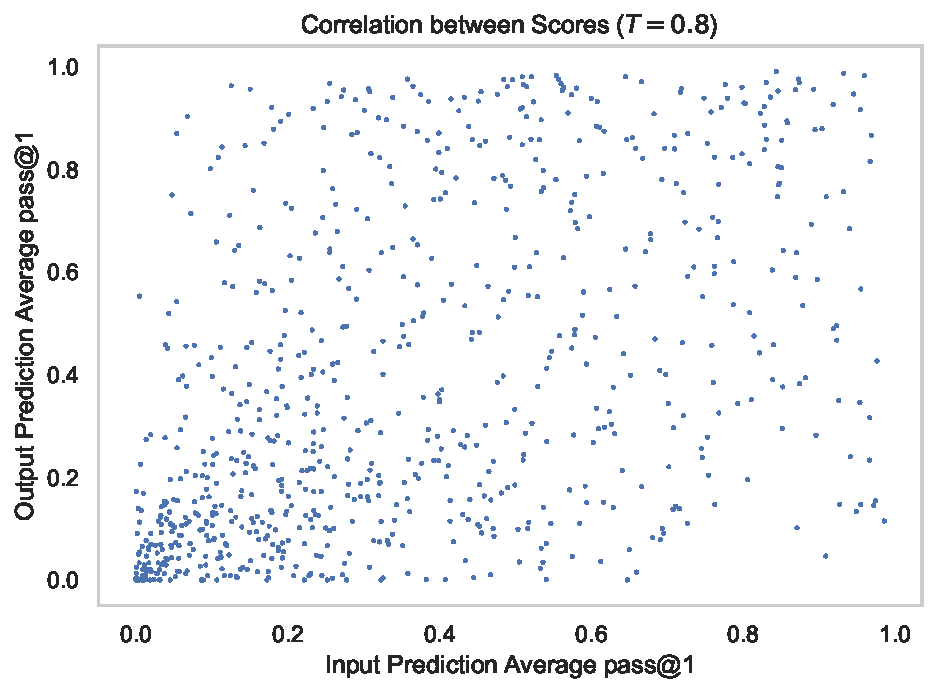
\includegraphics[width=\textwidth]{figs/benchmark/io_sample_correlation_0.8.pdf}
        \caption{$T=0.8$}
    \end{subfigure}
    \caption{Sample-by-sample correlation between Input Prediction and Output Prediction}
    \label{fig:benchmark-sample-io-correlation}
\end{figure}

\textbf{Method-level statistics}: In Fig. \ref{fig:benchmark-method-statistics}, we show the number of samples containing each method in \texttt{str, list}, and \texttt{dict}. Even though we distilled the same number of samples using each \texttt{str} function and about twice as many for each \texttt{list} and \texttt{dict} functions, we observe that the resulting distribution is highly non-uniform. This is due to a few reasons. First, about 30\% of the time, \codellamalarge sometimes fails to follow the instruction of including the library method in the resulting function. Second, some functions naturally lead to more operations that are removed by the filter. Third, common functions such as \texttt{str/list.index} or \texttt{list.append} are used in methods they are not prompted in. 

\begin{figure}[H]
    \centering
    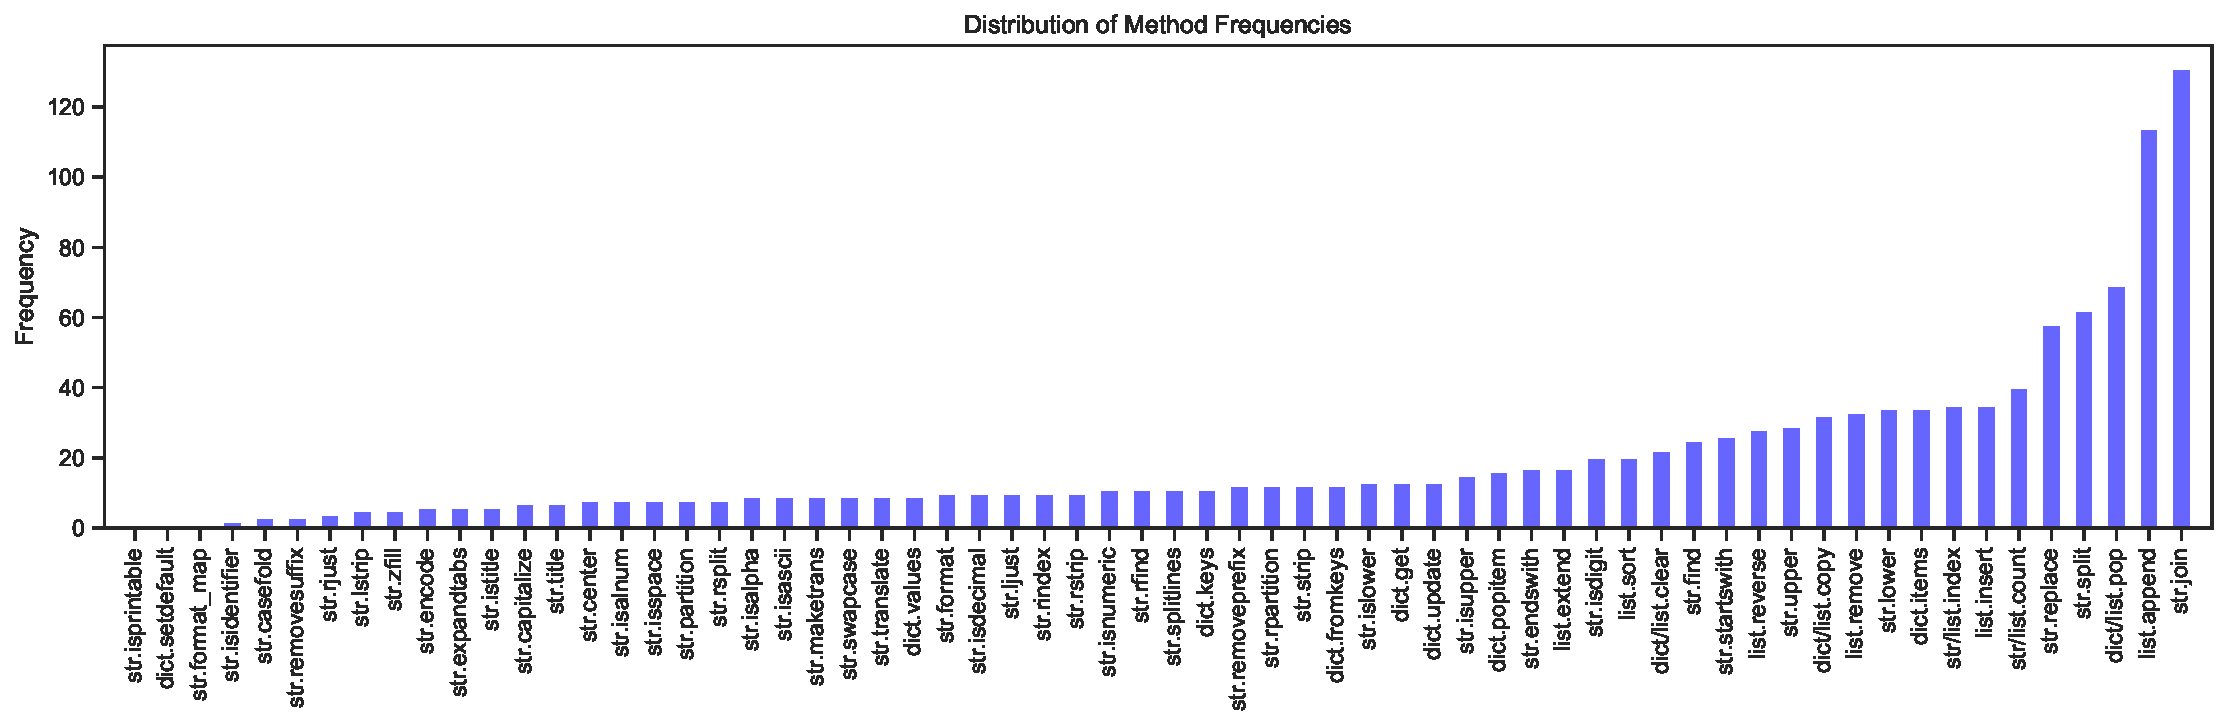
\includegraphics[width=\textwidth]{figs/benchmark/dataset_method_frequencies.pdf}
    \caption{Frequency of various methods in \benchmark}
    \label{fig:benchmark-method-statistics}
\end{figure}

Next, we investigate trends of which methods are easier/harder for code LMs. For each method in the \texttt{list}, \texttt{str}, and \texttt{dict} libraries listed in Appendix \ref{appendix:benchmark-generation-functions} with at least 5 samples, we calculate the average input prediction and output prediction score of benchmark samples containing that method. We show the 7 easiest and hardest methods for Code Llama 34B (Fig. \ref{fig:dataset-difficult-cl}), WizardCoder 34B (Fig. \ref{fig:dataset-difficult-wizardcoder}), and GPT-4 (Fig. \ref{fig:dataset-difficult-gpt4}). Some of the hardest methods, such as \texttt{str.rsplit, str.maketrans, str.rfind}, seem to be more obscure. We hypothesize that they may be underrepresented in pretraining corpora, explaining models' worse performance. While the distilled datasets of models like Phi, Phind, and WizardCoder are not yet available to the public, we speculate that they may include of fewer instances of these underrepresented functions and that distilling more obscure methods may help the model better learn their syntax and semantics.

\begin{figure}[H]
    \centering
    \begin{subfigure}[b]{0.49\textwidth}
        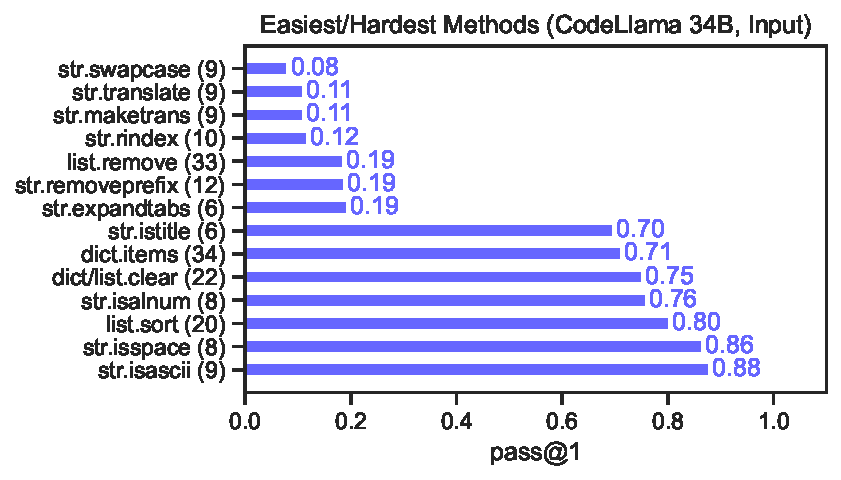
\includegraphics[width=\textwidth]{figs/benchmark/dataset_difficult_methods_codellama_input.pdf}
        \caption{Input Prediction}
    \end{subfigure}
    \begin{subfigure}[b]{0.49\textwidth}
        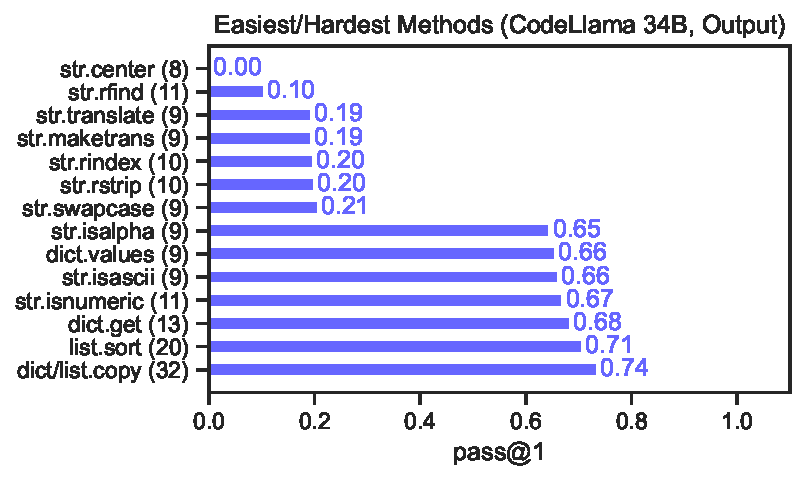
\includegraphics[width=\textwidth]{figs/benchmark/dataset_difficult_methods_codellama_output.pdf}
        \caption{Output Prediction}
    \end{subfigure}
    \caption{Easiest and hardest methods for Code Llama 34B input and output prediction, by pass@1 score ($T=0.2$)}
    \label{fig:dataset-difficult-cl}
\end{figure}

\begin{figure}[H]
    \centering
    \begin{subfigure}[b]{0.49\textwidth}
        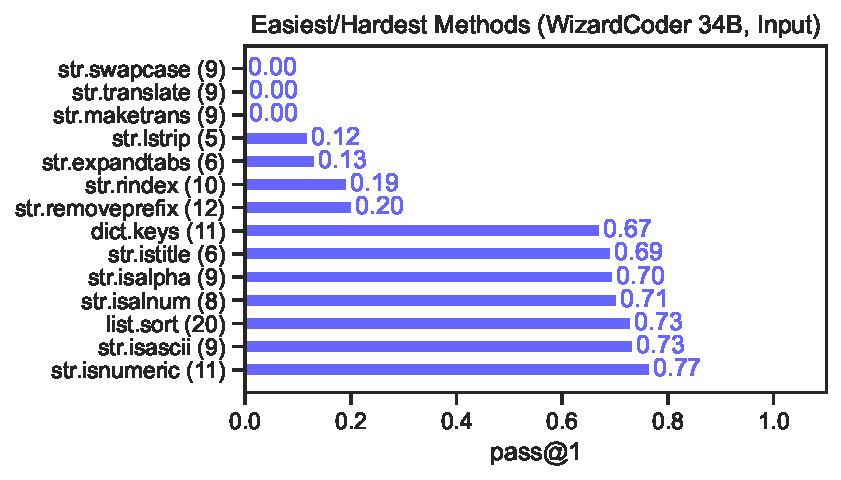
\includegraphics[width=\textwidth]{figs/benchmark/dataset_difficult_methods_wizardcoder_input.pdf}
        \caption{Input Prediction}
    \end{subfigure}
    \begin{subfigure}[b]{0.49\textwidth}
        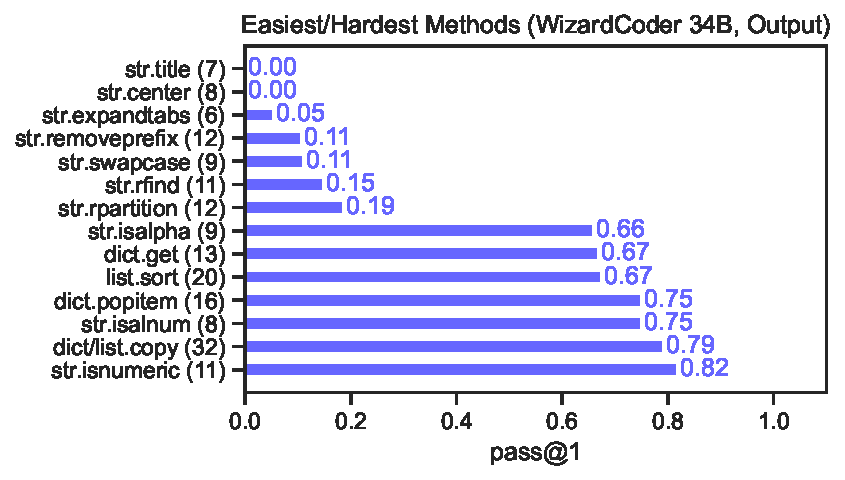
\includegraphics[width=\textwidth]{figs/benchmark/dataset_difficult_methods_wizardcoder_output.pdf}
        \caption{Output Prediction}
    \end{subfigure}
    \caption{Easiest and hardest methods for WizardCoder 34B input and output prediction, by pass@1 score ($T=0.2$)}
    \label{fig:dataset-difficult-wizardcoder}
\end{figure}

\begin{figure}[H]
    \centering
    \begin{subfigure}[b]{0.49\textwidth}
        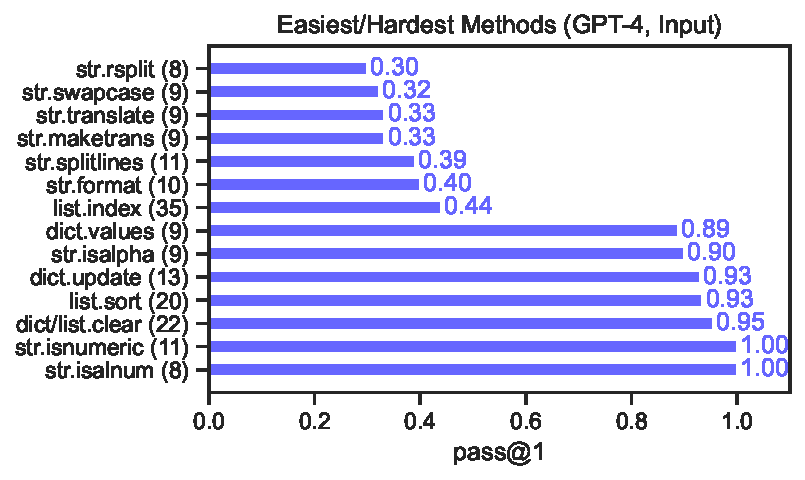
\includegraphics[width=\textwidth]{figs/benchmark/dataset_difficult_methods_gpt4_input.pdf}
        \caption{Input Prediction}
    \end{subfigure}
    \begin{subfigure}[b]{0.49\textwidth}
        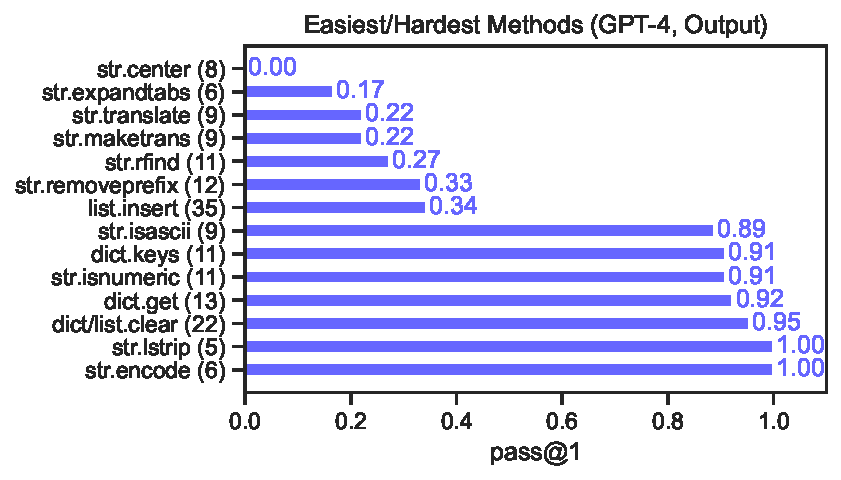
\includegraphics[width=\textwidth]{figs/benchmark/dataset_difficult_methods_gpt4_output.pdf}
        \caption{Output Prediction}
    \end{subfigure}
    \caption{Easiest and hardest methods for Code Llama 34B input and output prediction, by pass@1 score ($T=0.2$)}
    \label{fig:dataset-difficult-gpt4}
\end{figure}